\documentclass[10pt,a4paper,onecolumn]{article}
% \usepackage[utf8]{inputenc}
\usepackage{marginnote}
\usepackage{graphicx}
\usepackage{xcolor}
\usepackage{authblk,etoolbox}
\usepackage{titlesec}
\usepackage{calc}
\usepackage{hyperref}
\hypersetup{breaklinks=true,
            bookmarks=true,
            pdfauthor=
{
      Alexandra K. Diem,
  },
            pdftitle=
{
[Re] Chemical Signalling in the Neurovascular Unit
},
            colorlinks=true,
            citecolor=blue,
            urlcolor=blue,
            linkcolor=blue,
            pdfborder={0 0 0}}
\urlstyle{same}
\usepackage{tcolorbox}
\usepackage{ragged2e}
\usepackage{fontspec}
\usepackage{fontawesome}
\usepackage{caption}
\usepackage{listings}
\lstnewenvironment{code}{\lstset{language=Haskell,basicstyle=\small\ttfamily}}{}



%\usepackage{fancyvrb}
%\VerbatimFootnotes
%\usepackage{graphicx}
%\usepackage{mdframed}
%\newmdenv[backgroundcolor=lightgray]{Shaded}


\usepackage{longtable,booktabs}

\usepackage[
  backend=biber,
%  style=alphabetic,
%  citestyle=numeric
]{biblatex}
\bibliography{bibliography.bib}

\usepackage{amsmath,amssymb}



% --- Macros ------------------------------------------------------------------
\renewcommand*{\bibfont}{\small \sffamily}

\definecolor{red}{HTML}{CF232B}
\newcommand{\ReScience}{Re{\bfseries \textcolor{red}{Science}}}

\newtcolorbox{rebox}
   {colback=blue!5!white, colframe=blue!40!white,
     boxrule=0.5pt, arc=2pt, fonttitle=\sffamily\scshape\bfseries,
     left=6pt, right=20pt, top=6pt, bottom=6pt}

\newtcolorbox{repobox}
   {colback=red, colframe=red!75!black,
     boxrule=0.5pt, arc=2pt, left=6pt, right=6pt, top=3pt, bottom=3pt}

% fix for pandoc 1.14     
\newcommand{\tightlist}{%
  \setlength{\itemsep}{1pt}\setlength{\parskip}{0pt}\setlength{\parsep}{0pt}}

% --- Style -------------------------------------------------------------------
\renewcommand*{\bibfont}{\small \sffamily}
\renewcommand{\captionfont}{\small\sffamily}
\renewcommand{\captionlabelfont}{\bfseries}

\makeatletter
\renewcommand\@biblabel[1]{{\bf #1.}}
\makeatother

% --- Page layout -------------------------------------------------------------
\usepackage[top=3.5cm, bottom=3cm, right=1.5cm, left=1.5cm,
            headheight=2.2cm, reversemp, includemp, marginparwidth=4.5cm]{geometry}

% --- Section/SubSection/SubSubSection ----------------------------------------
\titleformat{\section}
  {\normalfont\sffamily\Large\bfseries}
  {}{0pt}{}
\titleformat{\subsection}
  {\normalfont\sffamily\large\bfseries}
  {}{0pt}{}
\titleformat{\subsubsection}
  {\normalfont\sffamily\bfseries}
  {}{0pt}{}
\titleformat*{\paragraph}
  {\sffamily\normalsize}


% --- Header / Footer ---------------------------------------------------------
\usepackage{fancyhdr}
\pagestyle{fancy}
%\renewcommand{\headrulewidth}{0.50pt}
\renewcommand{\headrulewidth}{0pt}
\fancyhead[L]{\hspace{-1cm}\includegraphics[width=4.0cm]{rescience-logo.pdf}}
\fancyhead[C]{}
\fancyhead[R]{} 
\renewcommand{\footrulewidth}{0.25pt}

\fancyfoot[L]{\hypersetup{urlcolor=red}
              \sffamily \ReScience~$\vert$
              \href{http://rescience.github.io}{rescience.github.io}
              \hypersetup{urlcolor=blue}}
\fancyfoot[C]{\sffamily 9 - \thepage}
\fancyfoot[R]{\sffamily  $\vert$
                        Volume 3 $\vert$
                        Issue 1}
\pagestyle{fancy}
\makeatletter
\let\ps@plain\ps@fancy
\fancyheadoffset[L]{4.5cm}
\fancyfootoffset[L]{4.5cm}

% --- Title / Authors ---------------------------------------------------------
% patch \maketitle so that it doesn't center
\patchcmd{\@maketitle}{center}{flushleft}{}{}
\patchcmd{\@maketitle}{center}{flushleft}{}{}
% patch \maketitle so that the font size for the title is normal
\patchcmd{\@maketitle}{\LARGE}{\LARGE\sffamily}{}{}
% patch the patch by authblk so that the author block is flush left
\def\maketitle{{%
  \renewenvironment{tabular}[2][]
    {\begin{flushleft}}
    {\end{flushleft}}
  \AB@maketitle}}
\makeatletter
\renewcommand\AB@affilsepx{ \protect\Affilfont}
%\renewcommand\AB@affilnote[1]{{\bfseries #1}\hspace{2pt}}
\renewcommand\AB@affilnote[1]{{\bfseries #1}\hspace{3pt}}
\makeatother
\renewcommand\Authfont{\sffamily\bfseries}
\renewcommand\Affilfont{\sffamily\small\mdseries}
\setlength{\affilsep}{1em}

\LetLtxMacro{\OldIncludegraphics}{\includegraphics}
\renewcommand{\includegraphics}[2][]{\OldIncludegraphics[width=12cm, #1]{#2}}


% --- Document ----------------------------------------------------------------
\title{[Re] Chemical Signalling in the Neurovascular Unit}

    \usepackage{authblk}
                        \author[1]{Alexandra K. Diem}
                            \affil[1]{Computational Engineering and Design, Faculty of Engineering and the
Environment, University of Southampton, Southampton, UK}
            
\date{\vspace{-5mm}
      \sffamily \small \href{mailto:alexandra.diem@gmail.com}{alexandra.diem@gmail.com}}


\setlength\LTleft{0pt}
\setlength\LTright{0pt}


\begin{document}
\maketitle

\marginpar{
  %\hrule
  \sffamily\small
  %\vspace{2mm}
  {\bfseries Editor}\\
  Benoît Girard\\

  {\bfseries Reviewers}\\
        Tiina Manninen\\
        Christoph Metzner\\
  
  {\bfseries Received}  Jun 20 2017\\
  {\bfseries Accepted}  Sept 06 2017\\
  {\bfseries Published} Sept 13 2017\\

  {\bfseries Licence}   \href{http://creativecommons.org/licenses/by/4.0/}{CC-BY}

  \begin{flushleft}
  {\bfseries Competing Interests:}\\
  The authors have declared that no competing interests exist.
  \end{flushleft}

  \hrule
  \vspace{3mm}

  \hypersetup{urlcolor=white}
  
    \vspace{-1mm}
  \begin{repobox}
    \bfseries\normalsize
      \href{http://github.com/ReScience-Archives/Diem-2017/tree/Diem-2017/article}{\faGithubAlt~Article repository}
  \end{repobox}
      \vspace{-1mm}
  \begin{repobox}
    \bfseries\normalsize
      \href{http://github.com/ReScience-Archives/Diem-2017/tree/Diem-2017/code}{\faGithubAlt~Code repository}
  \end{repobox}
      \vspace{-1mm}
  \begin{repobox}
    \bfseries\normalsize
      \href{http://github.com/ReScience-Archives/Diem-2017/tree/Diem-2017/data}{\faGithubAlt~Data repository}
  \end{repobox}
      \hypersetup{urlcolor=blue}
}

\begin{rebox}
\sffamily {\bfseries A reference implementation of}
\small
\begin{flushleft}
\begin{itemize}
    \item[→] Witthoft A, Karniadakis GE (2012) A bidirectional model for
communication in the neurovascular unit. \emph{Journal of Theoretical
Biology} 311: 80-93.
  \end{itemize}\par
\end{flushleft}
\end{rebox}


\section{Introduction}\label{introduction}

Witthoft and Karniadakis \autocite{Witthoft2012} introduced a model for
communication via chemical signalling within the neurovascular unit
(NVU). In the NVU neurons communicate their nutrient requirements to the
cerebral arteries via astrocytes \autocite{Nelson2015}: the activity of
neurons releases glutamate (Glu) and potassium (K\textsuperscript{+})
into the synaptic space, causing astrocytes to release potassium into
the periarterial space via their end-feet, leading to the activation of
smooth muscle cells (SMC) in the artery wall and thus a dilation of the
artery to increase blood flow.

Functional hyperemia is an important mechanism in the brain, by which an
increased neuronal metabolism leads to an increase of blood flow in
surrounding arteries in order to maintain adequate oxygen and nutrient
supply to the active neurons. This process works via a cascade of
chemical signalling processes from neurons to astrocytes to arteries.
The unidirectional vascular response to increased neuronal demands has
previously been modelled \autocite{Bennett2008}\autocite{Farr2011},
however, these models did not include the activity of the transient
receptor potential vanilloid-related channel 4 (TRPV4). The TRPV4
channel is a mechanosensitive calcium channel and leads to a
depolarisation of the astrocyte in response to the dilation of the
artery wall.

The paper \autocite{Witthoft2012} contains the differential equations
that are being modelled, however no code repository is provided. The
model is useful for the investigation of the effect of cerebrovascular
diseases on the brain and thus an openly available code repository
reproducing the results of this paper will be helpful to other
researchers.

\section{Methods}\label{methods}

The paper indicates that the original code was written in Matlab, while
the reproduction presented here is written in Python 3.5. The model is
given as a series of ordinary differential equations (ODE), which are
implemented as a function nvu(). This function is solved using the
scipy.integrate library. Initial attempts to solve the system of ODE
using the standard function odeint() failed. Instead, the equations can
be solved using the function ode() with the integration method set to
``lsoda'', which automatically selects between the Adams method for
non-stiff and BDF for stiff problems. The ODE system described in
\autocite{Witthoft2012} is a stiff system. Values for absolute and
relative tolerance have to be set in order for the simulation to finish
successfully. These are given in the results section as they differ for
different simulations. Future users of this code should note that the
simulation of a longer time span may require the use of different values
for absolute and relative tolerance, which have to be found via trial
and error, but from experience, they should not be larger than 1e-4 or
smaller than 1e-11.

The code was implemented following the descriptions of the equations in
\autocite{Witthoft2012}, but upon cross-checking equations against their
equivalents in
\autocite{Bennett2008}\autocite{Farr2011}\autocite{Gonzalez1994} it
became evident that some of the equations contain typographical errors.
This was confirmed after contacting the authors of
\autocite{Witthoft2012}. Changes to the equations are as follows:

\begin{itemize}
\item
  \begin{enumerate}
  \def\labelenumi{(\arabic{enumi})}
  \setcounter{enumi}{9}
  \tightlist
  \item
    \(J_{TRPV}\) should be positive, such that
    \(J_{TRPV} = I_{TRPV}/(C_{astr} \gamma)\).
  \end{enumerate}
\item
  \begin{enumerate}
  \def\labelenumi{(\arabic{enumi})}
  \setcounter{enumi}{19}
  \tightlist
  \item
    \(I_{\Sigma K}\) should be defined as
    \(I_{\Sigma K} = -J_{\Sigma K} C_{astr} \gamma\) (changed sign).
  \end{enumerate}
\item
  \begin{enumerate}
  \def\labelenumi{(\arabic{enumi})}
  \setcounter{enumi}{22}
  \tightlist
  \item
    \(J_{Ca}\) is not defined in the manuscript, but correspondence with
    the original authors revealed that it should be defined as
    \(J_{Ca} = -I_{Ca}/(C_{SMC} \gamma)\).
  \end{enumerate}
\item
  \begin{enumerate}
  \def\labelenumi{(\arabic{enumi})}
  \setcounter{enumi}{22}
  \tightlist
  \item
    Both \(J_{TRPV}\) and \(J_{Ca}\) should be divided by the volume
    ratios of perivascular to astrocyte and SMC space (analogous to
    equation (22)), such that it reads
    \[\frac{d \left[ Ca\textsuperscript{2+} \right] }{dt} = -\frac{J_{TRPV}}{VR_{pa}} - \frac{J_{Ca}}{VR_{ps}} - Ca_{decay} \left( \left[ Ca\textsuperscript{2+} \right]_p - \left[ Ca\textsuperscript{2+} \right]_{p,0} \right).\]
  \end{enumerate}
\item
  \begin{enumerate}
  \def\labelenumi{(\arabic{enumi})}
  \setcounter{enumi}{30}
  \tightlist
  \item
    \(I_K = g_K n (V_m - v_K)\) \autocite{Farr2011}.
  \end{enumerate}
\item
  (A.1) Term \(\frac{1}{2 \alpha} I_{Ca}\) should be \(\alpha I_{Ca}\)
  (to comply with code for \autocite{Witthoft2013} by the original
  authors) such that
  \[\frac{d \left[ Ca^{2+} \right]_{SMC}}{dt} = -\rho \left( \alpha I_{Ca} + k_{Ca} \left[ Ca^{2+} \right]_{SMC} \right).\]
\item
  (A.3) When implementing this equation it has to be multiplied by
  \(\mu\)m to get the correct units of force.
\item
  (A.6) The brackets around the exponential function are set
  incorrectly, it should read
  \[\sigma'_y = \frac{\sigma_{y_0}}{\sigma_0^\#} \frac{\exp \left( \frac{-(y' - y'_0)^2}{2 \left[ y'_1/(y' + y'_2) \right]^{2 y'_4}} \right) - y'_3}{1 - y'_3}\]
  \autocite{Gonzalez1994}.
\item
  Parameter \(C_{SMC}\) is given as \(C\) in Table B2 in
  \autocite{Witthoft2012}.
\item
  Decimal of parameter \(a\) in Table B2 in \autocite{Witthoft2012} is
  in the wrong place, it should read \(a = 502.65\) \(\mu\)m\(^2\).
\item
  Parameter \(P_L\) has units of \(\mu\)M instead of \(\mu\)M/s.
\item
  The value for {[}Ca\textsuperscript{2+}{]}\textsubscript{ER} is not
  given, but can be found in \autocite{Bennett2008} as
  {[}Ca\textsuperscript{2+}{]}\textsubscript{ER} \(= 400 \mu\)m.
\item
  Parameter \(g_{TRPV} = 50\) pS is incorrectly cited from
  \autocite{Kung2005}, correct value was found in the newer model
  \autocite{Witthoft2013}.
\item
  Parameter \(k_{Ca} = 135.68\) 1/s is incorrectly cited from
  \autocite{Gonzalez1994}.
\end{itemize}

\begin{figure}
\centering
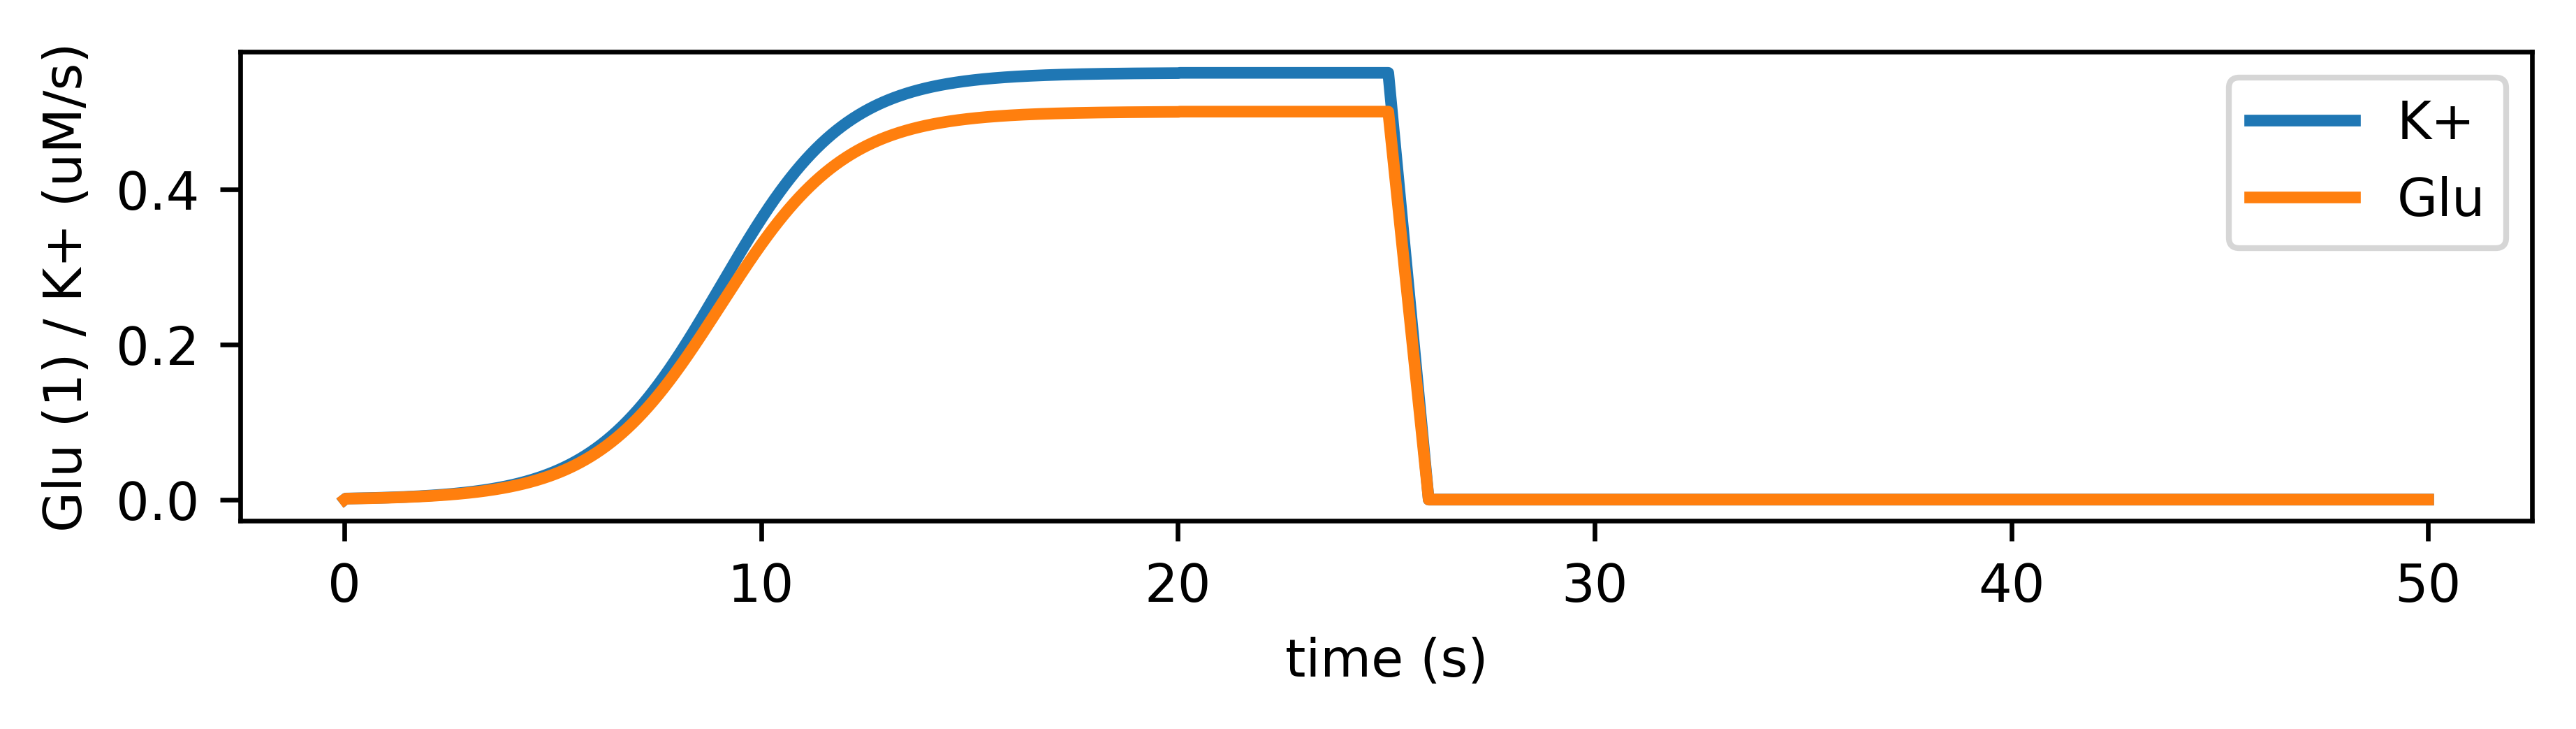
\includegraphics{figures/input.png}
\caption{Input functions for the NVU model. K+ (blue) refers to
potassium and Glu (orange) refers to glutamate released into the
synaptic space as a consequence of synaptic activity by the neuron.
Potassium levels are given in units of \(\mu\)M/s while the glutamate
value actually refers to the ratio of bound and unbound glutamate
receptors (equation (3) \autocite{Witthoft2012}) and is therefore
unitless. Maximum values were found by trial and error such that
potassium and IP\textsubscript{3} in Figure ~\ref{fig:fig1} here match
Figure 5 in the original publication.}\label{fig:input}
\end{figure}

The input to the model is not explictly provided in the original
publication, only the statement ``We simulated neural-induced
vasodilation by representing the total synaptic activity in the
astrocyte domain as a uniform, continuous smooth pulse of glutamate
(\(J_{K_s}\)) and of synaptic potassium
({[}K\textsuperscript{+}{]}\textsubscript{s}).'' is provided
\autocite{Witthoft2012}. Upon correspondence with the authors both
glutamate and synaptic potassium were modelled as a tanh function over
20 s to a maximum value of 0.55 uM/s for K\textsuperscript{+} and 0.5
for the ratio of bound/unbound Glu receptors, which was sustained for a
further 5 s, giving a total stimulus time of 25 s, followed by a linear
decrease to zero over 1 s. The functions for the input are

\[J_{K_s} = 0.55 \cdot \begin{cases} 0.5 \cdot (1 + \tanh((t-9)/3)) & \text{for } 0 \leq t \leq 20\\
1.0 & \text{for } 20 < t \leq 25\\
26 - t & \text{for } 25 < t \leq 26\\
0 & \text{otherwise}\end{cases}\]

and analogously for \(\rho\) in equation (3). Both are provided in the
code of this implementation and are shown in Figure ~\ref{fig:input}.
Maximum values were found by trial and error such that potassium and
IP\textsubscript{3} in Figure ~\ref{fig:fig1} here match Figure 5 in the
origial publication.

Furthermore, upon correspondence with the original authors, an
equilibration phase of 20 s before the simulation had to be implemented.
During the equilibration phase no glutamate or potassium is released
into the synaptic space and the solution values at the end of the
equilibration phase are used as initial values for the main simulation.
This step is not mentioned in the original publication, but is vital to
obtain the correct results.

\section{Results}\label{results}

Results from the code presented in this repository aim at reproducing
Figure 5 in the original application, which shows ion and voltage
dynamics over a simulation period of 50 s.

\begin{figure}
\centering
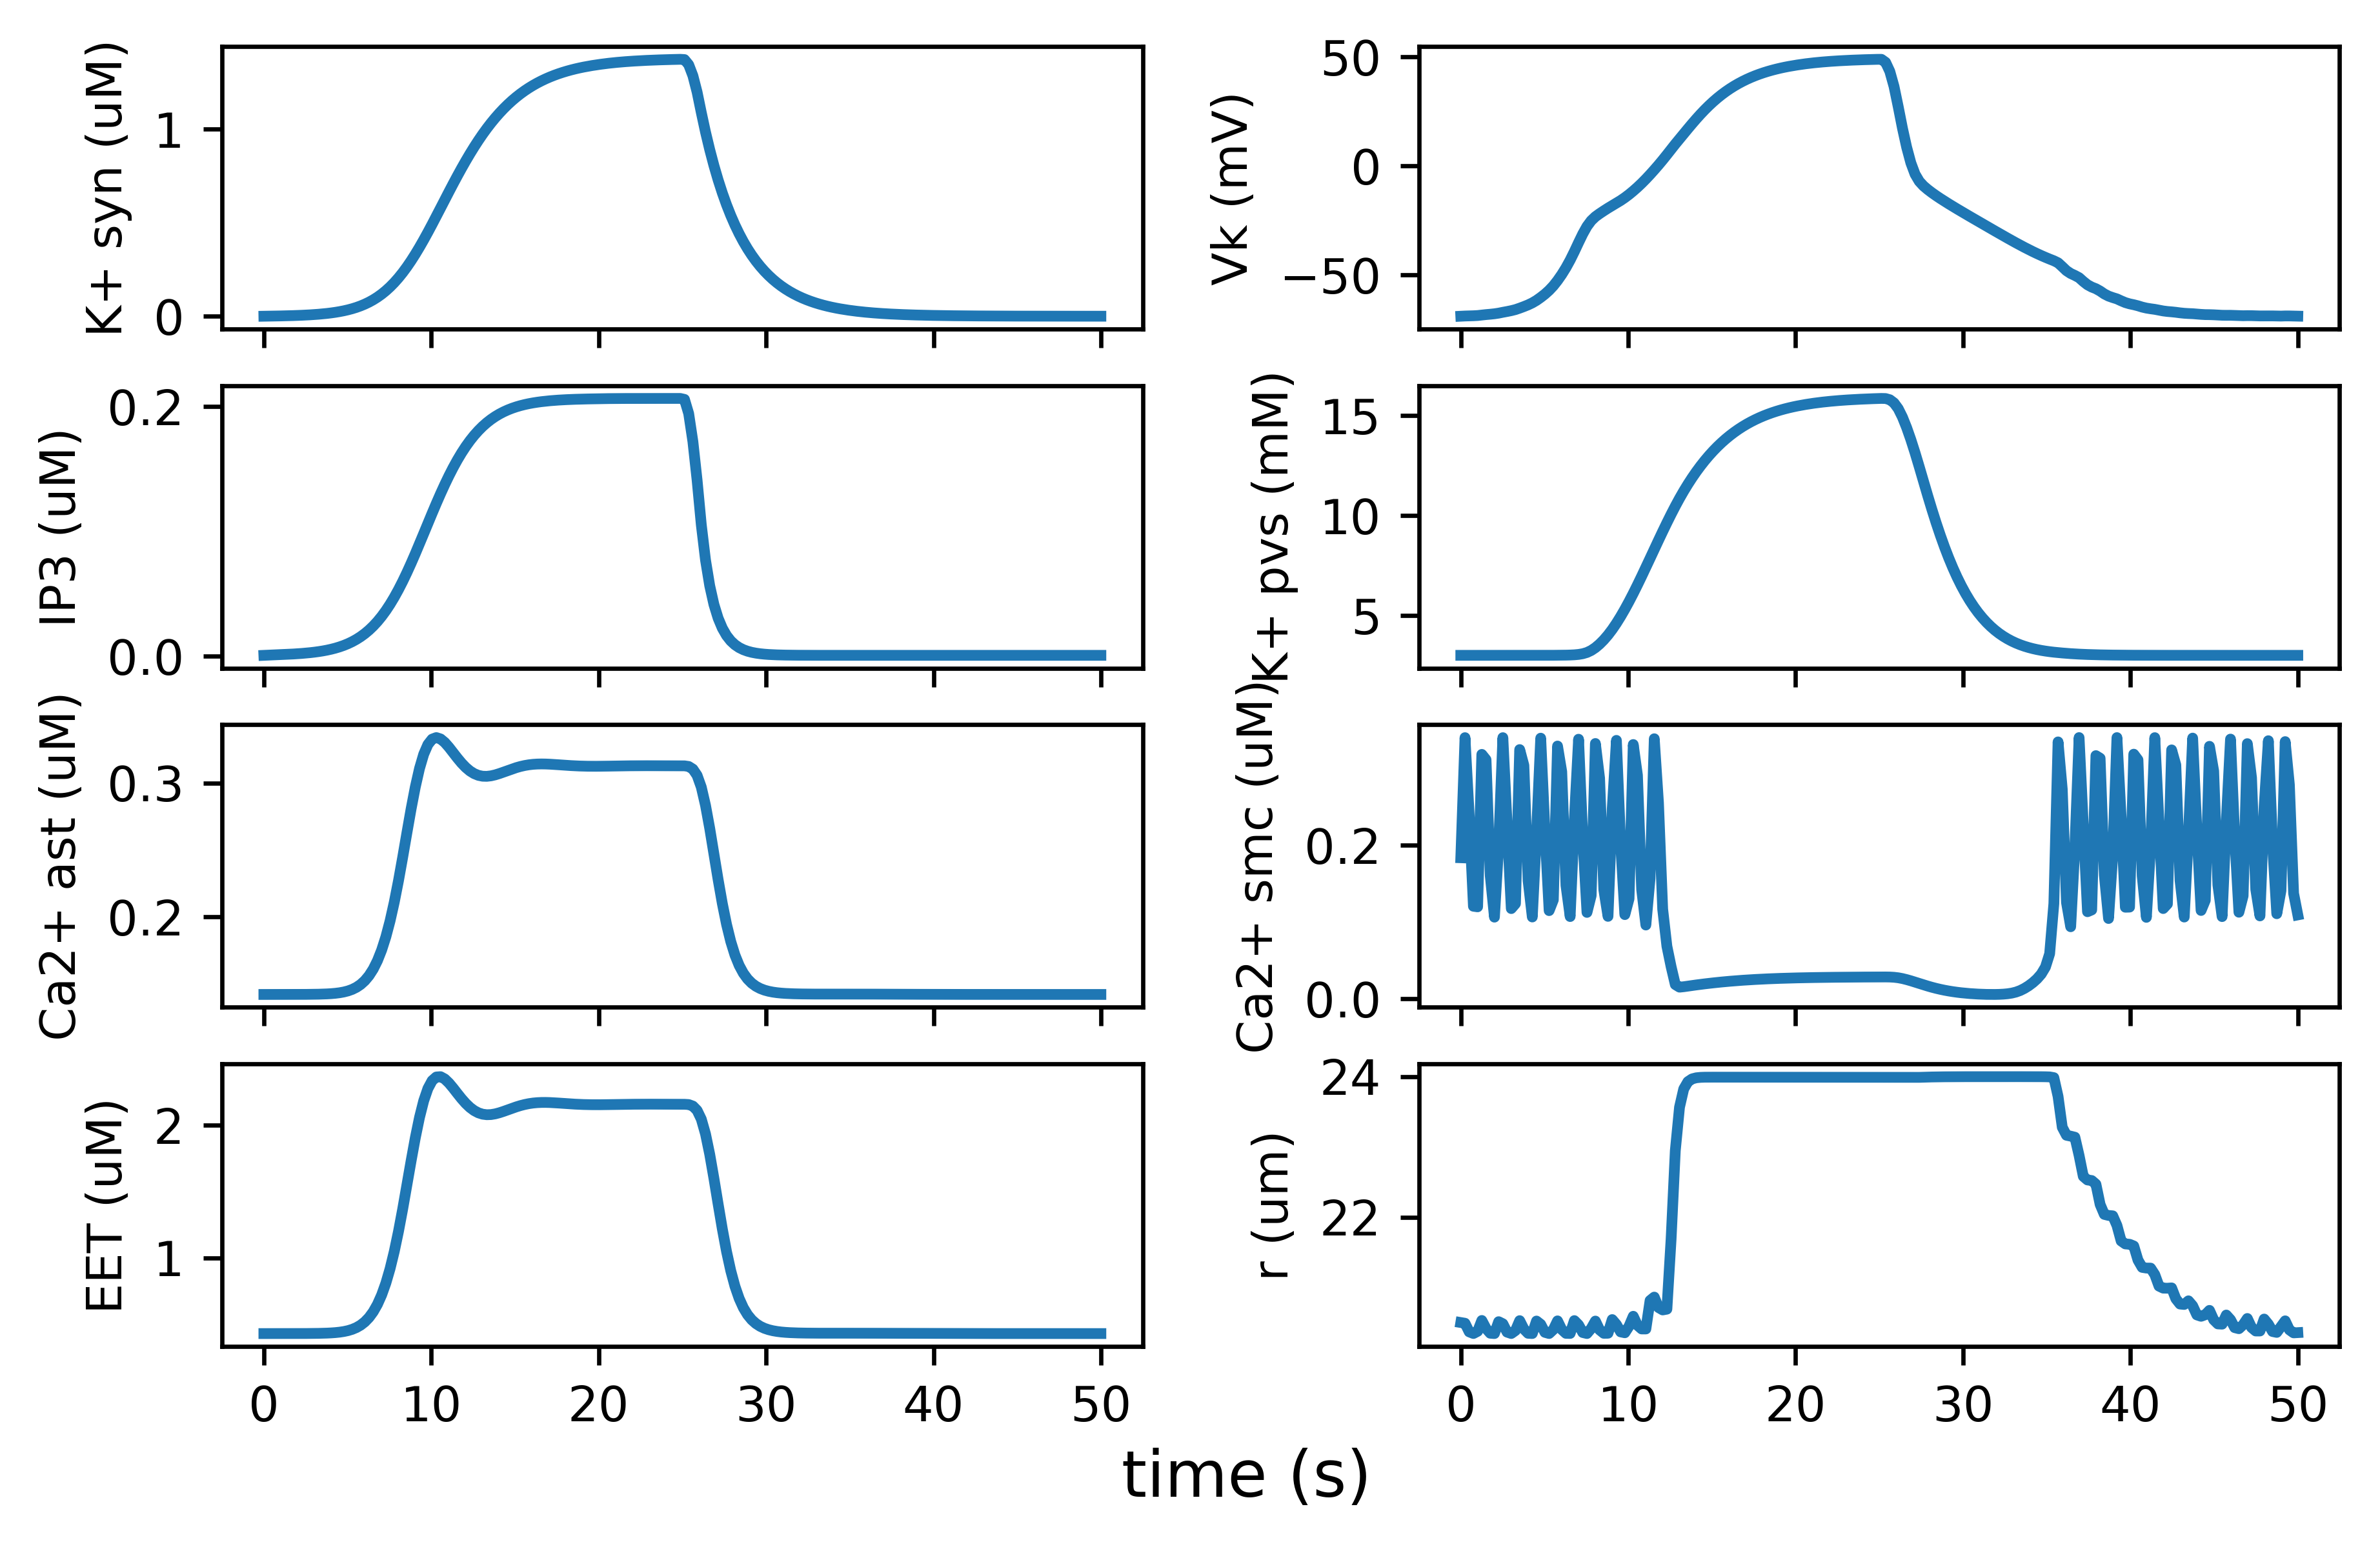
\includegraphics{figures/fig1.png}
\caption{Astrocyte and arterial response during neuronal stimulation.
This figure is a reproduction of Figure 5 in the original publication
using the code in this repository. The dashed black line shows the model
without TRPV channels. Potassium (K\textsuperscript{+}) in both the
synaptic and perivascular space match their corresponding plots in the
original publication, as do calcium (Ca\textsuperscript{2+}) in the
smooth muscle cell and the arterial radius. Differences can be seen for
the astrocyte membrane potential V\textsubscript{k}. Most interesting is
the shape of V\textsubscript{k}, which in the first half looks very
different from the reproduced figure. Additionally, V\textsubscript{k}
overshoots into positive values, which is not given in the original
publication. Simulation tolerance values atol=1e-8,
rtol=1e-7.}\label{fig:fig1}
\end{figure}

Figure ~\ref{fig:fig1} shows the results obtained from replicating
Figure 5 in the original publication (main.py). Potassium
(K\textsuperscript{+}) in both the synaptic and perivascular space match
their corresponding plots in the original publication, as do calcium
(Ca\textsuperscript{2+}) in the smooth muscle cell and the arterial
radius. Differences can be seen for the astrocyte membrane potential
V\textsubscript{k} and the perivascular K\textsuperscript{+}
concentration. Most interesting is the shape of V\textsubscript{k},
which in the first half looks very different from the reproduced figure.
The depolarisation as well as the relaxation after stimulus removal
appear to occur much faster compared to the original publication. The
depolarisation shows a small dip at around 7 s. Additionally,
V\textsubscript{k} overshoots into positive values, which is not given
in the original publication. Perivascular K\textsuperscript{+} does not
reach 20 mM as in the original publication, which may be a result of the
other differences.

The large difference in V\textsubscript{k} between the two simulations
is surprising, especially because this does not lead to incorrect
results in the other plots. The key results, which are the response of
Ca\textsuperscript{2+} and subsequently the arterial radius match the
original publication. A newer publication by the same authors exists
\autocite{Witthoft2013}, which does contain a higher spike for
Ca\textsuperscript{2+} and epoxyeicosatrienoic acid (EET) as the
simulation results presented here. It is unclear, where this difference
comes from as \autocite{Witthoft2013} does not indicate that any of the
equations affecting Ca\textsuperscript{2+} or EET have been altered. It
is also unclear why V\textsubscript{k} shows such a large difference.

\begin{figure}
\centering
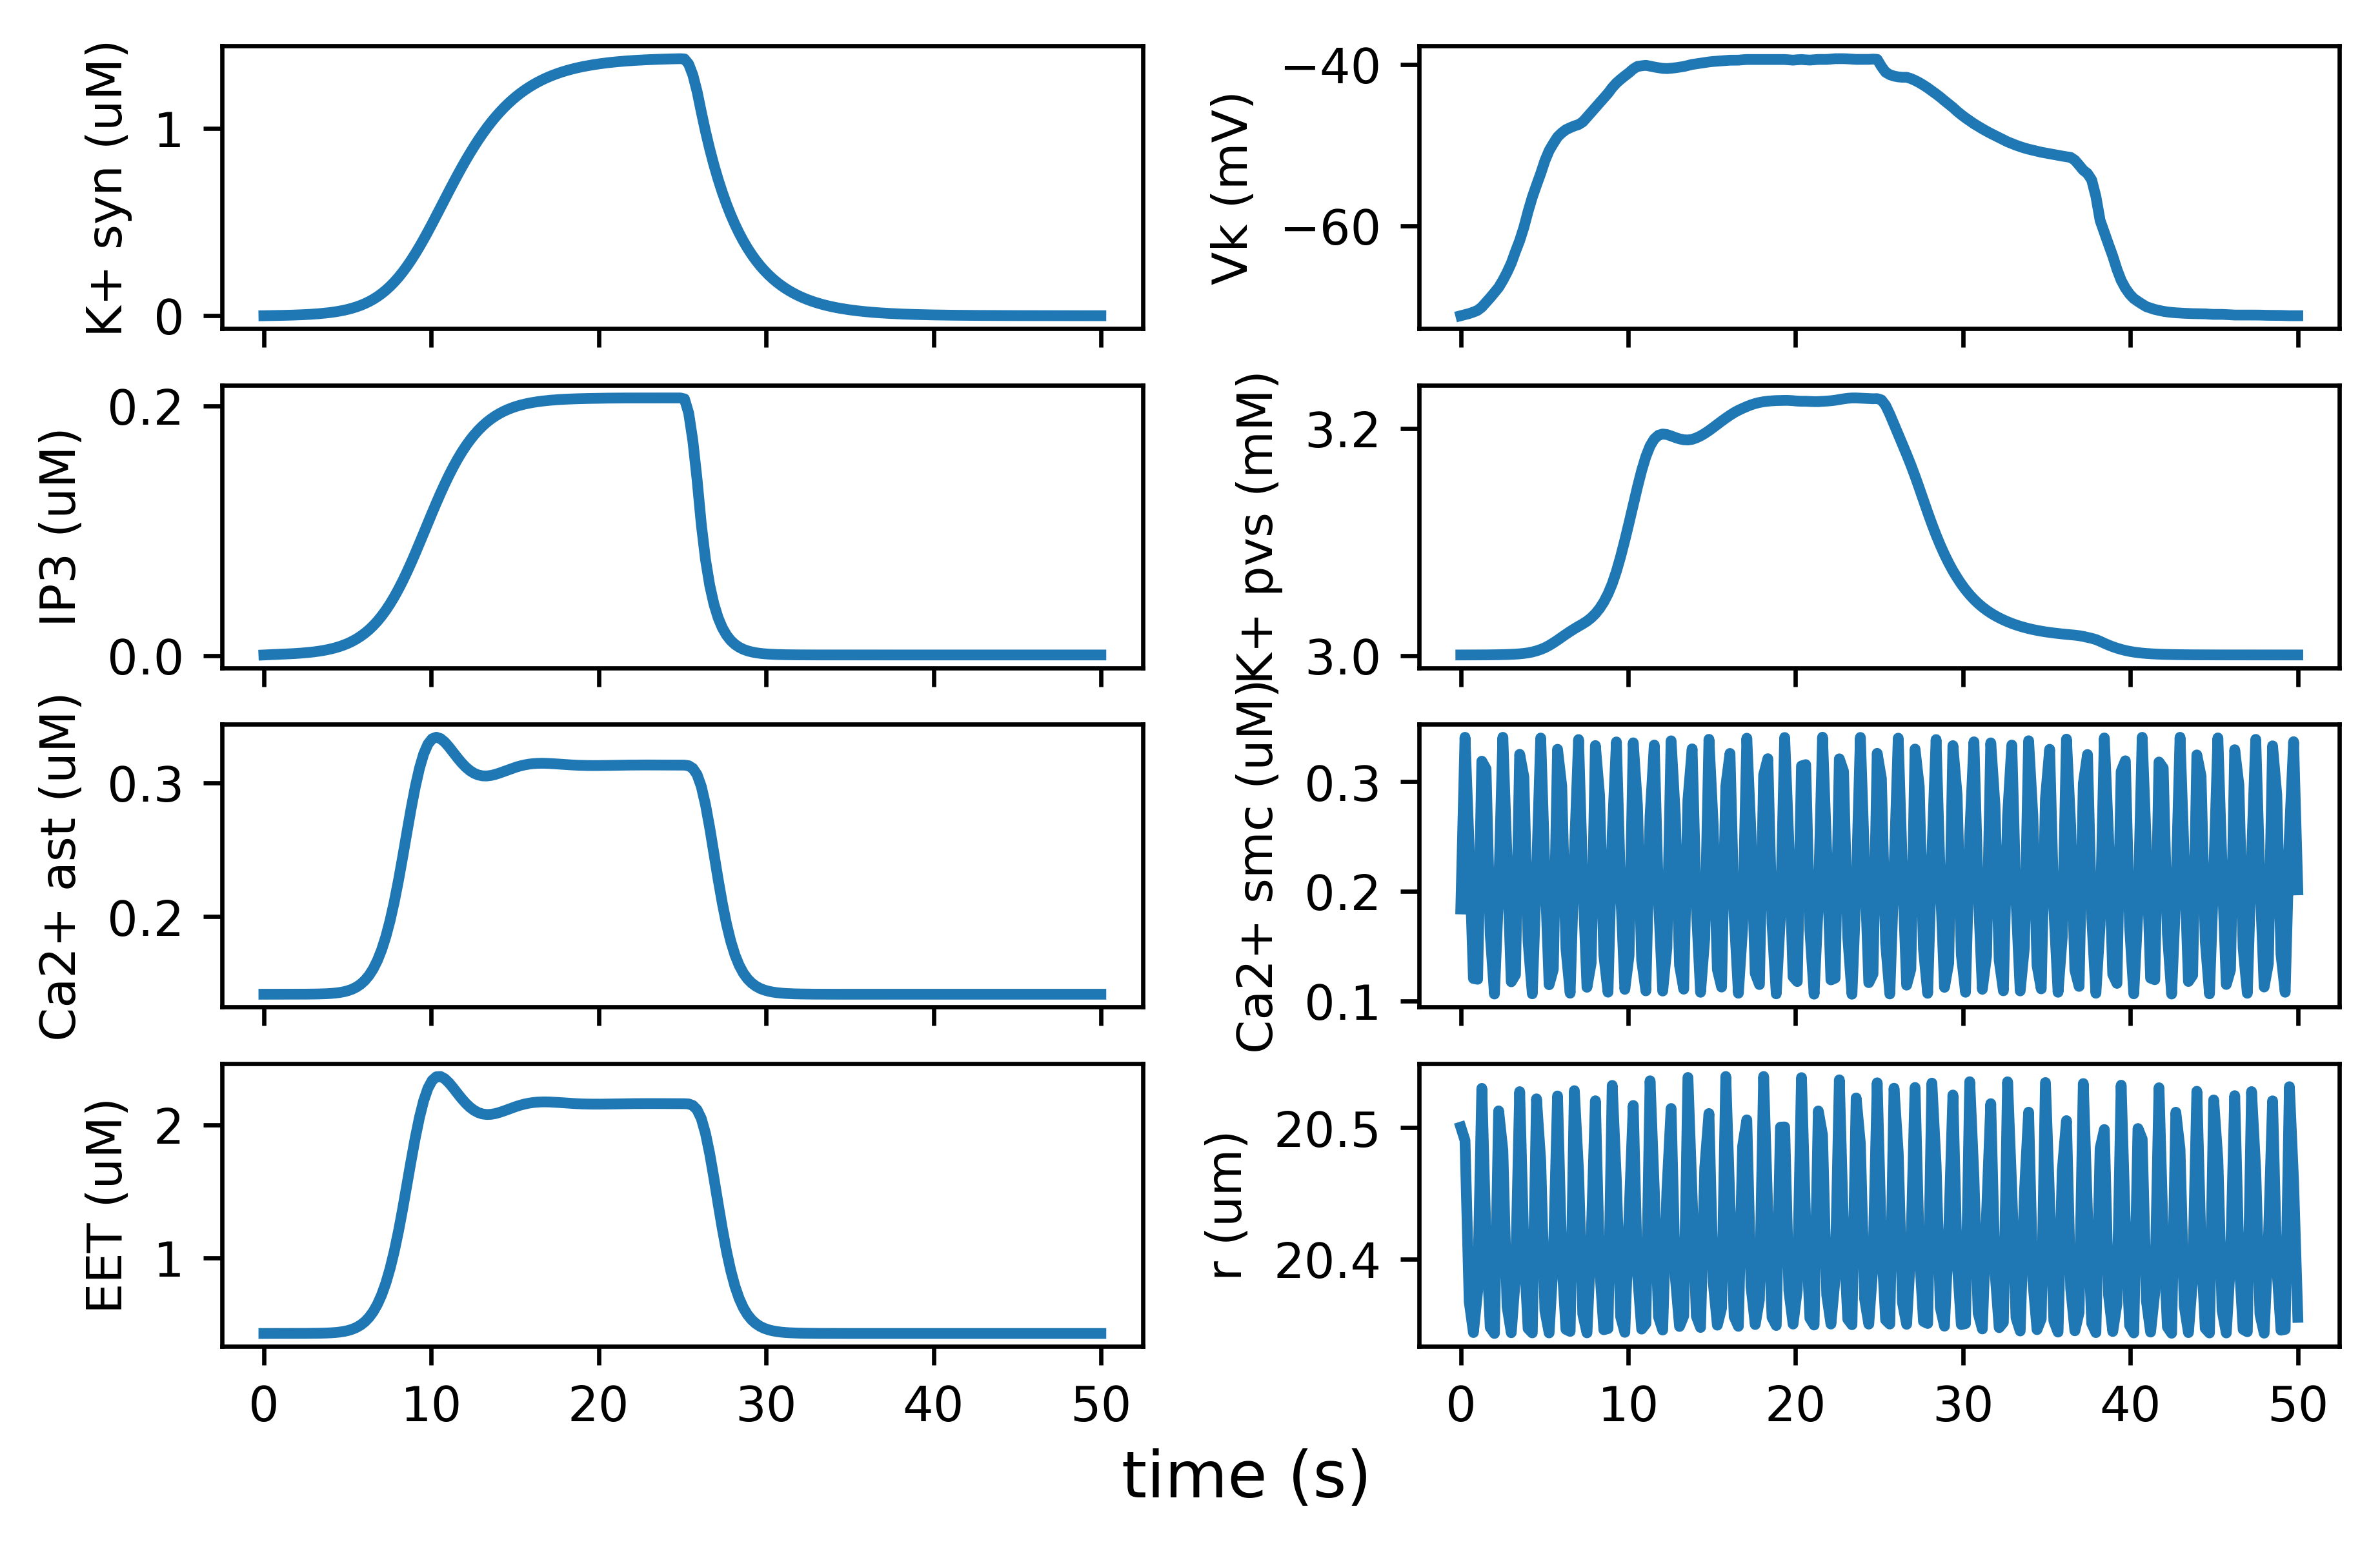
\includegraphics{figures/fig2.png}
\caption{Astrocyte and arterial response during neuronal stimulation
whilst V\textsubscript{k} is fixed to match the original publication.
The difference in results for K\textsuperscript{+} in the perivascular
space, Ca\textsuperscript{2+} in the smooth muscle cell and arterial
radius suggest that possible further errors in the equations exist in
the original publication. Simulation tolerance values atol=1e-7,
rtol=1e-7.}\label{fig:fig2}
\end{figure}

One possible explanation could be that some components of
\(\partial V_k / \partial t\) are wrongly implemented, but the results
are mostly affected by the mere fact that V\textsubscript{k} increases
in response to the stimulus instead of the exact value of
V\textsubscript{k}. To test this, V\textsubscript{k} was obtained from
the original publication and hard-coded into the simulation instead of
being calculated from its ODE (main\_Vk.py). This is shown in Figure
~\ref{fig:fig2}. Here, the results for K\textsuperscript{+} in the
perivascular space, Ca\textsuperscript{2+} in the smooth muscle cells
and the arterial radius differ largely from the results in the original
publication or indeed Figure ~\ref{fig:fig1}. Because of this
discrepancy between results the authors of the original publication were
contacted to request the code for this publication. However, they could
only provide the Matlab code for \autocite{Witthoft2013}, from which it
was not possible to revert back to the code to implement
\autocite{Witthoft2012}. Attempts were made to remove the additional
equations introduced in \autocite{Witthoft2013} from this code in order
to revert it back to what it might have been at the time of publication
of \autocite{Witthoft2012}. However, the results did not match. The
original authors were asked for advice, but stated that it would likely
be impossible to revert the code back to its original version due to the
sensitivity of parameters, which would make this processes immensely
error prone.

\begin{figure}
\centering
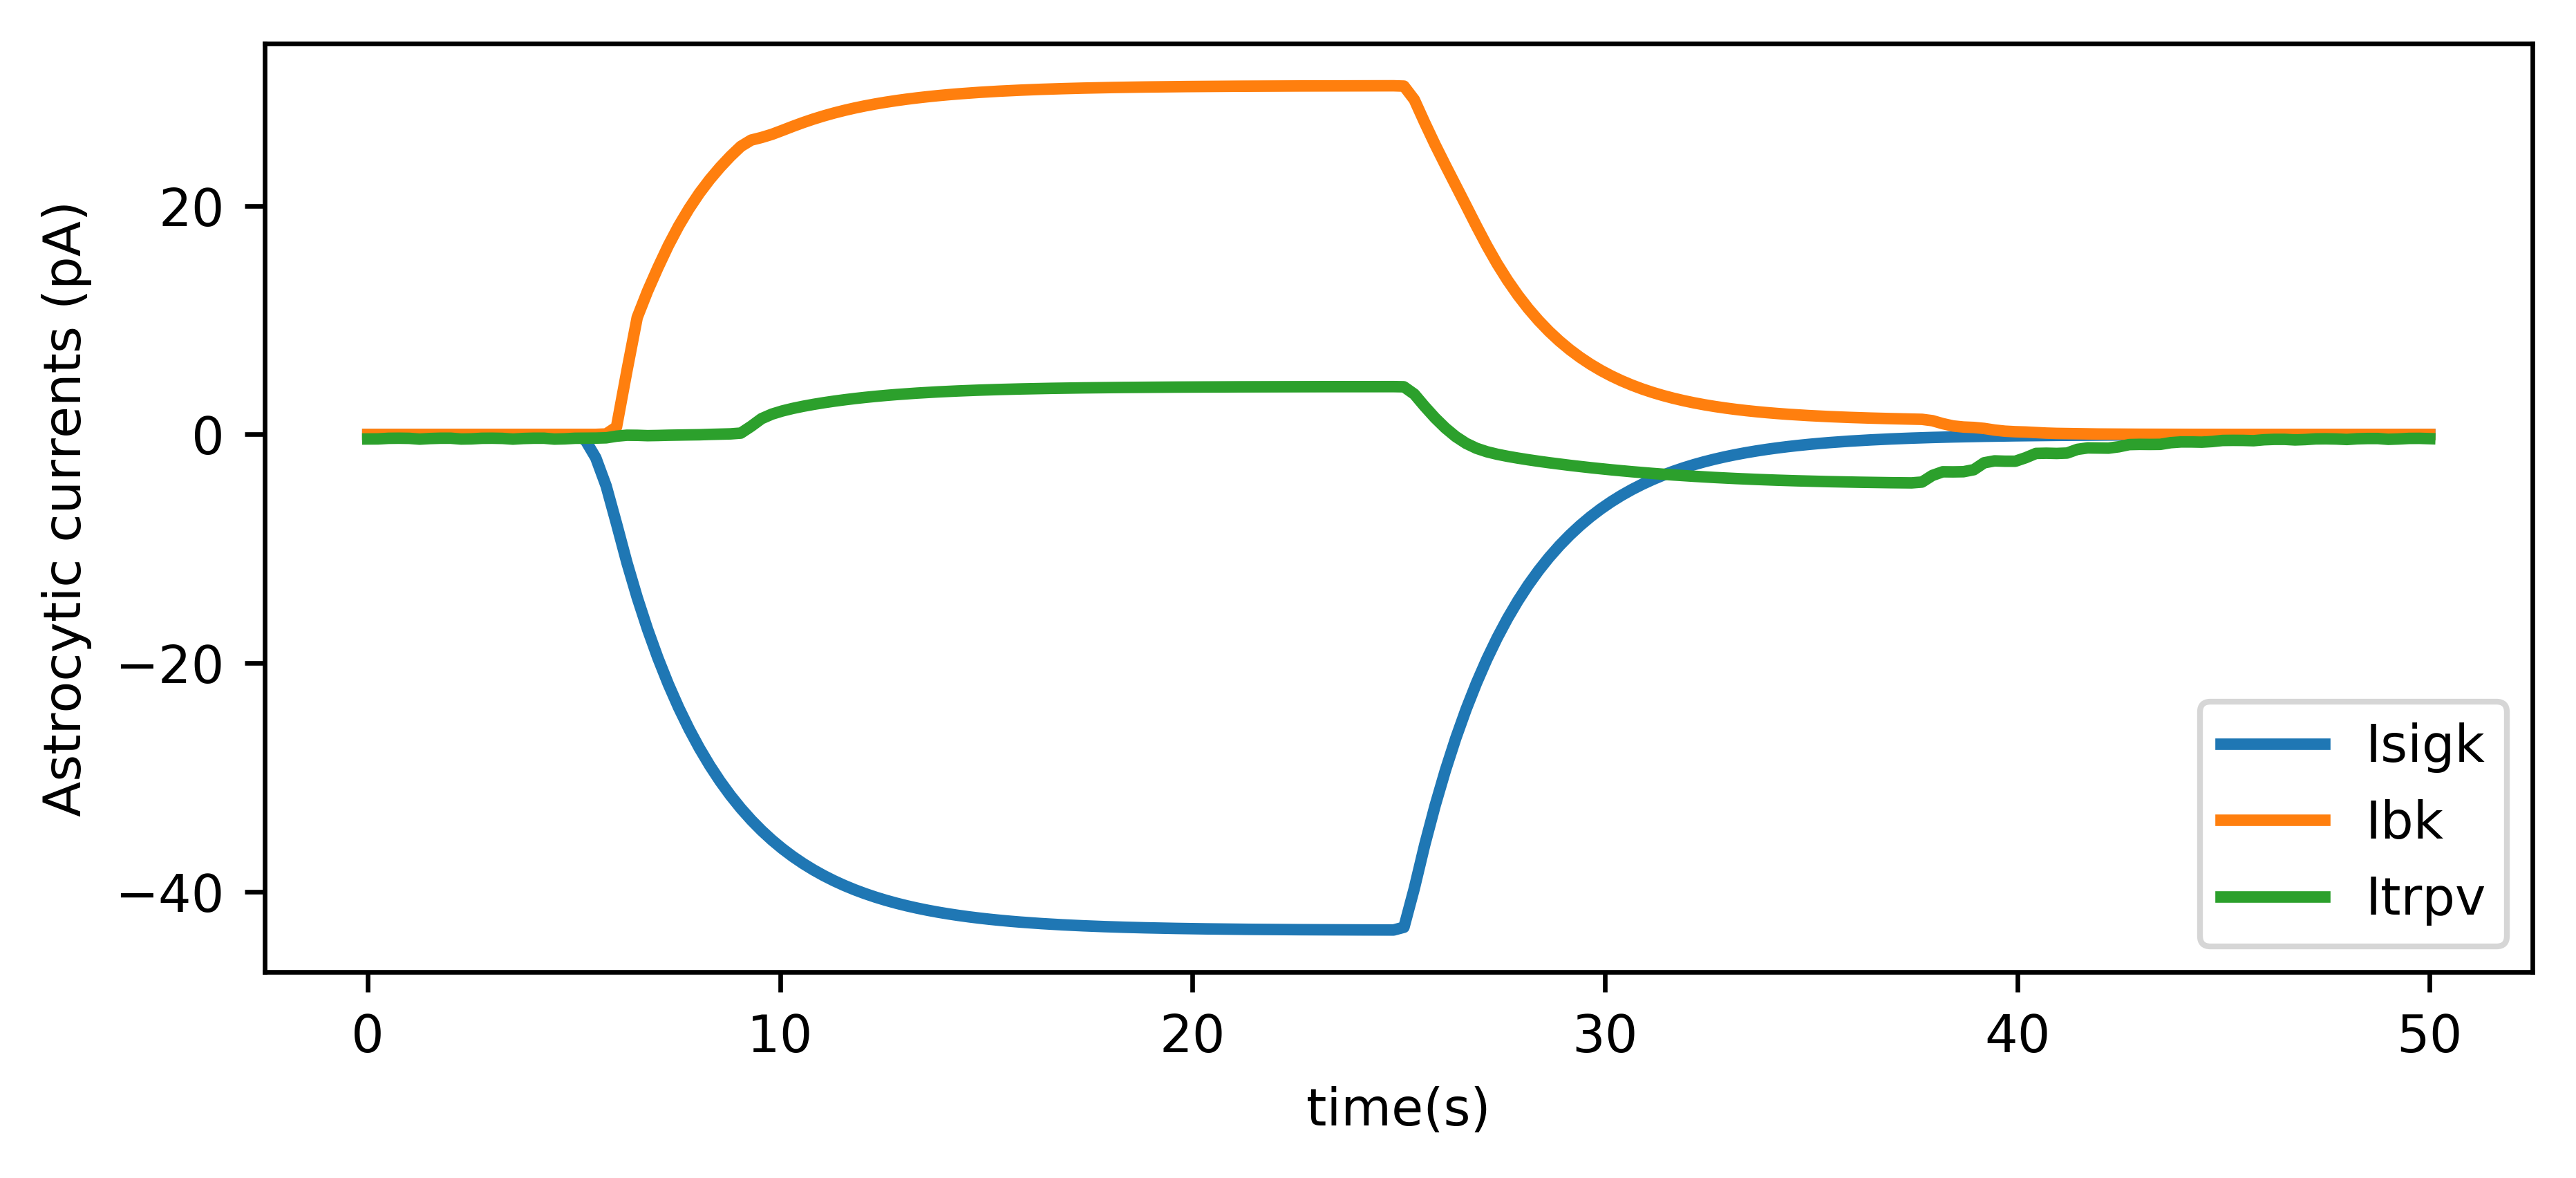
\includegraphics{figures/astr_currents.png}
\caption{Astrocyte currents from equation (20). Comparing the astrocyte
currents here to the ones presented in Figure S2 in
\autocite{Witthoft2013} shows discrepancies. The shape of Isigk
(\(I_{\Sigma K}\), equation 20) matches (note that the widths of the
figures differ), however its values differ by an order of magnitude. Ibk
(equation 15) appears to mostly match its equivalent in Figure S2, but
the numbers are two orders of magnitude larger. The shape of Itrpv shows
similarities, but larger by at least an order of magnitude, more likely
close to two.}\label{fig:astr_currents}
\end{figure}

The supplementary information of the newer publication
\autocite{Witthoft2013} contains plots of the astrocyte currents, which
may help to find the differences between this implementation and
\autocite{Witthoft2012} (Figure S2 \autocite{Witthoft2013}, Figure
~\ref{fig:astr_currents}). Comparing the astrocyte currents here to the
ones presented in Figure S2 in \autocite{Witthoft2013} shows
discrepancies. The shape of \(I_{\Sigma K}\) (equation 20) matches (note
that the widths of the figures differ), however its values differ by an
order of magnitude. \(I_{BK}\) (equation 15) appears to mostly match its
equivalent in Figure S2, but the numbers are two orders of magnitude
larger. The shape of Itrpv shows similarities, but larger by at least an
order of magnitude, more likely close to two. Figure S2 in
\autocite{Witthoft2013} contains additional KIR channel currents at the
astrocyte, which are not included in the original paper. Vice versa, the
leak channel equation has been removed in the newer model (most likely
because this has been replaced by two explicit KIR channel equations).
Thus, these are not plotted in Figure ~\ref{fig:astr_currents}.
\(I_{\Sigma K}\) is mostly defined by the values for potassium in the
synaptic space (equation 2). Because there is a discrepancy of the
synaptic potassium values by three orders of magnitude between the two
publications by Witthoft et al., this is the likely source for the
discrepancy in values for \(I_{\Sigma K}\). Only small differences exist
in the parameter definitions for \(I_{BK}\), but the size of the
discrepancy between the two models also suggests that it may arise from
the difference in potassium values at the input of the model. These
differences make a direct comparisons between astrocyte currents
difficult at best. Unfortunately, no results for the currents on the
smooth muscle cell membrane (\(V_m\), equation 30) are provided in
either publication.

\begin{figure}
\centering
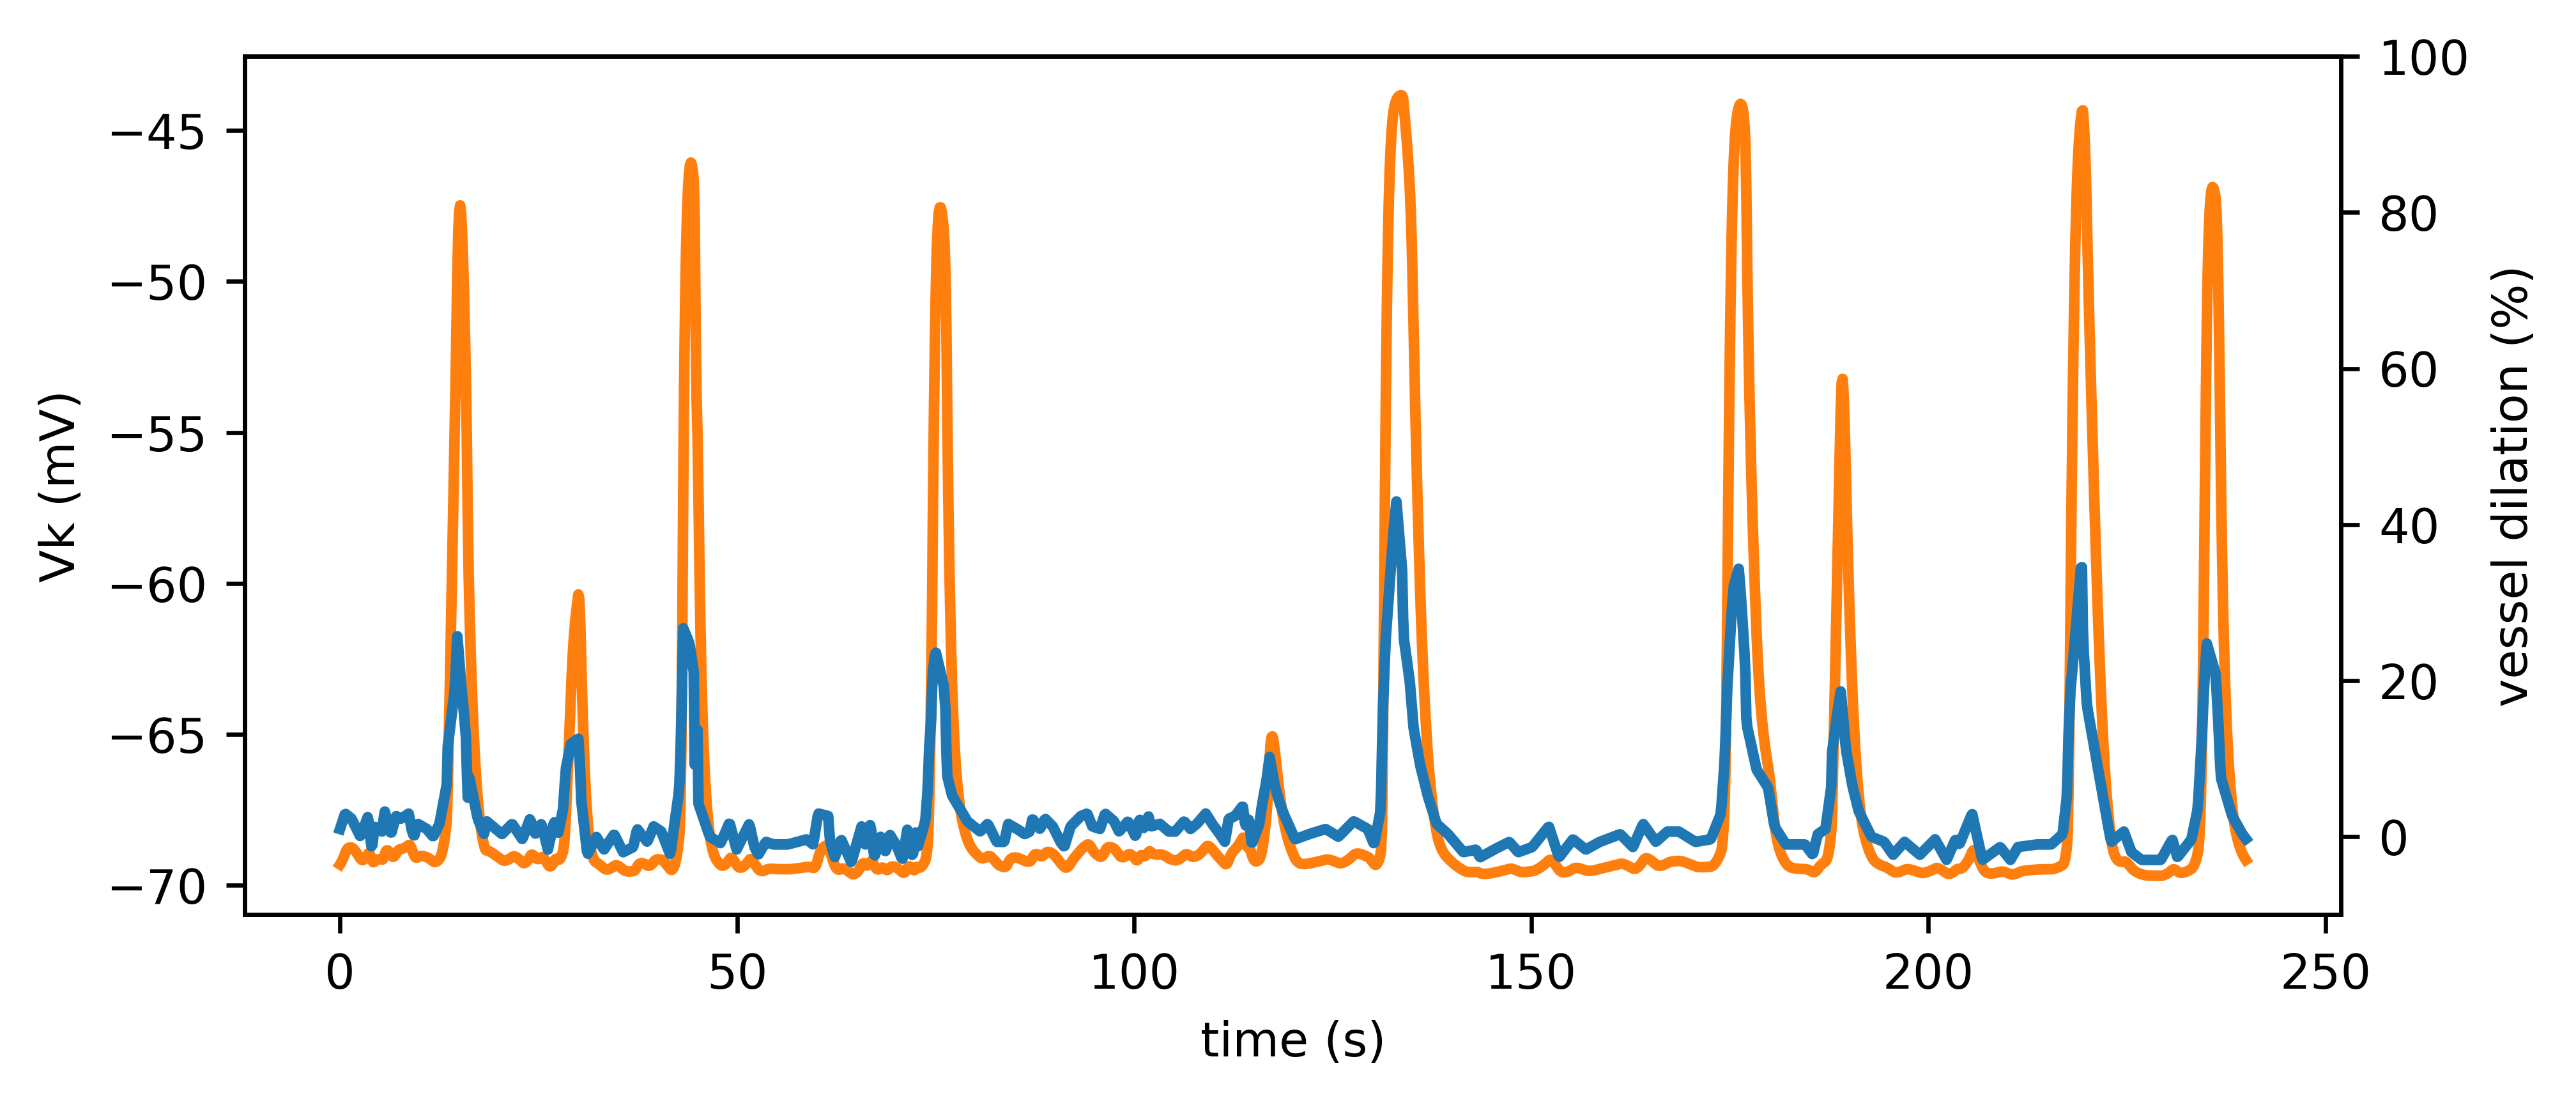
\includegraphics{figures/Vk_inflation.png}
\caption{Astrocyte membrane potential (orange) due to quick manual
inflation of the artery (blue). The experimental data describing the
artery stretch was obtained from \autocite{Witthoft2012} and originates
from \autocite{Cao2011}, compare to Figure 3 in \autocite{Witthoft2012}.
The astrocyte membrane potential was expected to range from -80 mV to
-40 mV and its decay was expected to be slower. Simulation tolerance
values atol=1e-7, rtol=1e-8.}\label{fig:vk_inflation}
\end{figure}

The original publication contains results to validate their TRPV model
equations (Figure 3 \autocite{Witthoft2012}). They obtained data of the
astrocyte membrane potential (Vk) of an artery being inflated by 20-40\%
of its original size in quick bursts \autocite{Cao2011}. The data of the
stretching of the vessel was extracted from \autocite{Witthoft2012} and
supplied as an input (variable \(x\)) to the NVU model (main\_trpv.py).
Figure ~\ref{fig:vk_inflation} shows the equivalent of Figure 3 in the
original publication. The figures compare well to some degree, however,
the astrocyte membrane potential appears to decay too quickly in this
simulation. Additionally, the value range does not match, which should
be -75 mV to -40 mV in the original publication, while it is
approximately -68 mV to -25 mV here. Tests to vary the parameters of
equation (23), which governs the change in perivascular calcium, did not
yield further improvements.

\begin{figure}
\centering
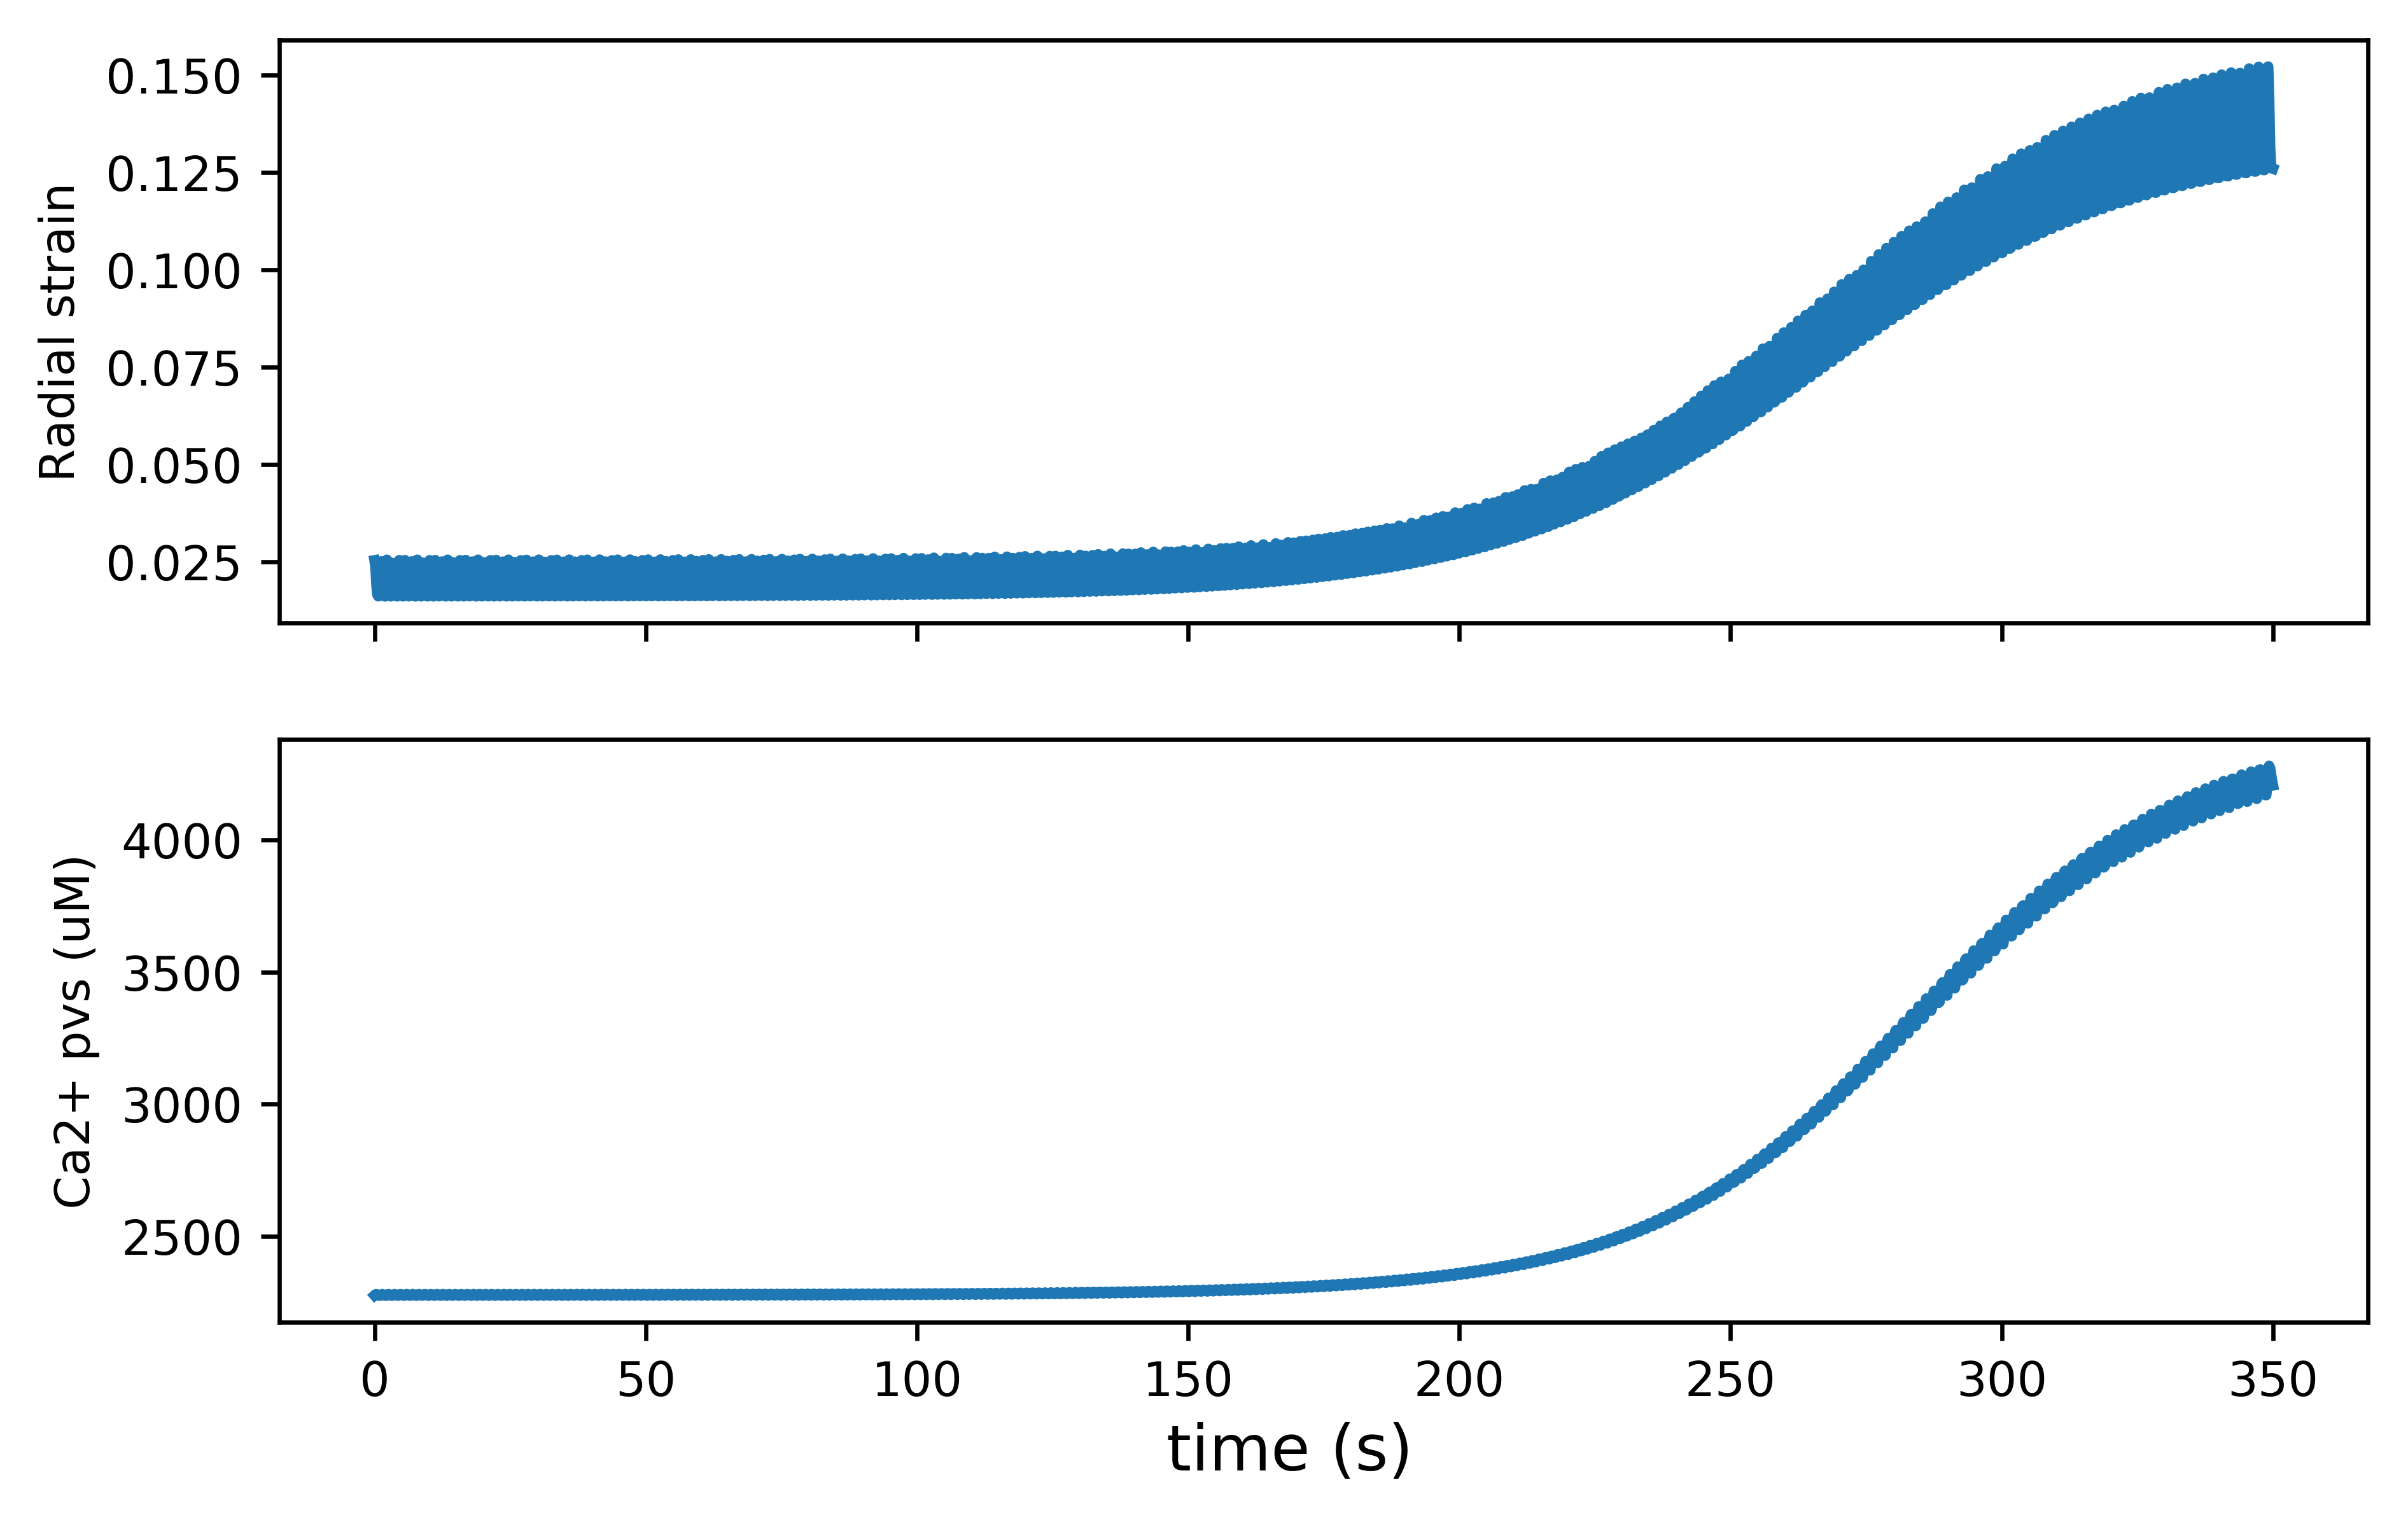
\includegraphics{figures/pinacidil_2000uM.png}
\caption{Effect of the vasodilatory drug pinacidil on the results.
Compare to Figure 4 in \autocite{Witthoft2012}. Radial strain appears to
be a good match, although its increase starts later compared to the
results in the original publication. The values for perivascular calcium
are much higher than in the original publication, but the reason for
this could not be found. Simulation tolerance values atol=1e-7,
rtol=1e-7.}\label{fig:pinacidil}
\end{figure}

Finally, the original publication contains results to investigate the
effect of the vasodilatory drug pinacidil (Figure 4
\autocite{Witthoft2012}). This was achieved by setting the variable
\(k\) to a set time course:

\[k(t) = 0.01 \left( 1 + \tanh \frac{t-270}{60} \right).\]

The results of this modification (main\_k.py) are shown in Figure
~\ref{fig:pinacidil}. Radial strain appears to be a good match, although
its increase starts later compared to the results in the original
publication. The values for perivascular calcium are much higher than in
the original publication, but the reason for this could not be found.

\section{Conclusion}\label{conclusion}

To a large degree the results from \autocite{Witthoft2012} were
replicated. However, distinct differences in the results remain, which
could not be explained. It should be emphasised that the number of
errors found in the original publication may indicate that more errors
may remain to be found, however, because no version of the code to
implement \autocite{Witthoft2012} appears to exist anymore, it will be
very difficult at best to find these additional errors.

{\sffamily \small
  \printbibliography[title=References]
}
\end{document}
